\documentclass{article}
\usepackage{tabularx,fullpage,url}
\usepackage[top=1in, bottom=1in, left=.5in, right=.75in]{geometry}
\usepackage{amsmath,amssymb,graphicx,amsthm,xparse, color, mathrsfs} 
\usepackage{ epstopdf, fullpage}


\newcommand{\mypagebreak}{\begin{center}
		\noindent\makebox[\linewidth]{\rule{7.5in}{1pt}}
	\end{center}}
	
	
	
\newcommand{\R}{\mathbb R}
\newcommand{\idx}[1]{_{[#1]}}
\newcommand{\mS}{\mathcal S}
\newcommand{\bmat}{\left[\begin{matrix}}
\newcommand{\emat}{\end{matrix}\right]}
\newcommand{\range}{\mathbf{range}}
\newcommand{\vnull}{\mathbf{null}}
\newcommand{\minimize}[1]{\underset{#1}{\text{minimize}}}
\newcommand{\mB}{\mathcal B}
\newcommand{\diag}{\mathbf{diag}}




\newcommand{\showpoints}[1]{(\textbf{#1})}


\begin{document}
{\Large\textbf{CSE 512: Homework  \hfill
Due Wednesday, October 6 }}


\mypagebreak


\section*{Extra practice problems, ungraded}
\begin{enumerate}
\item \emph{Gradients.}  Compute the gradients of the following functions. Give the exact dimension of the output.

\begin{enumerate}
\item \emph{Linear regression.}  $f(x) = \frac{1}{40}\|Ax-b\|_2^2$, $A\in \R^{20\times 10}$

\item \emph{Sigmoid.} $f(x) = \sigma(c^Tx)$, $c\in \R^5$, $\sigma(s) = \frac{1}{1+\exp(-x)}$.
Hint: Start by showing that $\sigma'(s) = \sigma(s)(1-\sigma(s))$.

\end{enumerate}
\item  \emph{Convex or not convex. } Are the following sets convex or not convex? Justify your answer.

\begin{enumerate}
\item $\mS =\range(A) := \{x : Az = x \text{ for some }z\}$




\item $\mS = \{x : x \leq -1\} \cup \{x : x \geq 1\}$ (Read: either $x \leq -1$ or $x \geq 1$.)

\end{enumerate}



\item \emph{Am I positive semidefinite?}   A symmetric matrix $X$ is \emph{positive semidefinite} if for all $u$, $u^TXu \geq 0$. For each of the following, either prove that the matrix is positive semidefinite, or find a counterexample. 

\begin{enumerate}
\item 
$
X = \bmat 
1 & 1 & 1 \\ 1& 1 & 1 \\ 1 & 1& 1
\emat
$



\item 
$
X = \bmat 
-1 & -1 & -1 \\ -1& 1 & -1 \\ -1 & -1& 1
\emat
$







\end{enumerate}



\item  \emph{Convex or not convex.} \showpoints{1pt, 0.125 points each.}
From lecture, we know that there are three ways of checking whether a function is convex or not.
\begin{itemize}
\item For any function, we can check if it satisfies the \textbf{definition of convexity}:
\[
f(\theta x + (1-\theta) y) \leq \theta f(x) + (1-\theta) f(y), \quad \forall x,y, \quad \forall 0\leq \theta \leq 1.
\]
\item For any differentiable function, we can check the \textbf{first-order condition}
\[
f(x)-f(y) \geq \nabla f(y)^T(x-y).
\]
\item For any twice-differentiable function, we can check the \textbf{second-order condition}
\[
\nabla^2 f(x) \text{ is positive semidefinite, i.e. } u^T\nabla^2 f(x) u \geq 0 \quad \forall u.
\]
\end{itemize}
Use any of these ways to determine whether or not each function is convex. (You only need to use one of these rules per function. Pick the one you think gets you to the answer the fastest!)

\begin{enumerate}
\item $f(x) = \frac{1}{2}(x\idx{1}^2-2x\idx{1}x\idx{2}+x\idx{2}^2)$



\item $f(x) = |x|$ Hint: Again, remember the triangle inequality.



 
\item $f(x) = \log(\exp(x\idx{1})+\exp(x\idx{2}))$


\item $f(x) = c^Tx$


\end{enumerate}



\end{enumerate}


\section*{Main assignment, graded}
\begin{enumerate}


\item \emph{Gradient properties.} \showpoints{1 pt, 0.5 pts each.} Prove the following two properties of gradients:
\begin{enumerate}
\item \emph{Linearity.} If $h(x) = \alpha f(x) + \beta g(x)$, then 
$\nabla h(x) = \alpha \nabla f(x) + \beta \nabla g(x).$


\item \emph{Chain rule.} Show that if $g(v) = f(Av)$, then $\nabla g(v) = A^T\nabla f(Av)$.


\end{enumerate}

\item \emph{Gradients.} \showpoints{1 pts, 0.5 pts each.}  Compute the gradients of the following functions. Give the exact dimension of the output.

\begin{enumerate}

\item \emph{Quadratic function.}  $f(x) = \frac{1}{2}x^TQx + p^Tx + r$, $Q\in \R^{12\times 12}$ and $Q$ is symmetric ($Q\idx{i,j} = Q\idx{j,i}$).

\item \emph{Softmax function.} $f(x) =\frac{1}{\mu} \log(\sum_{i=1}^8 \exp(\mu x\idx{i}))$, $x\in \R^8$, $\mu$ is a positive scalar

\end{enumerate}




\item  \emph{Convex or not convex. } \showpoints{1pt} Are the following sets convex or not convex? Justify your answer.

\begin{enumerate}
\item \showpoints{0.3 pts} $\mS = \{x : \sum_i x_i = 0\}$




\item \showpoints{0.2 pts} $\mS = \{(x,y) : x^2+y^2 = 1\}$



\item \showpoints{0.2 pts} $\mS = \{x : |x| \leq 1\}$.
Hint: Remember the triangle inequality.



\end{enumerate}

\item \emph{Am I positive semidefinite?} \showpoints{1 pt, 0.5 pts each}  A symmetric matrix $X$ is \emph{positive semidefinite} if for all $u$, $u^TXu \geq 0$. For each of the following, either prove that the matrix is positive semidefinite, or find a counterexample. 

\begin{enumerate}
\item 
$
X = \bmat 
1 & 2 & 3 \\ 2& 1 & 4 \\ 3 & 4 & 1
\emat
$




 \item $
X = \bmat 
1 & 0 & 0 \\ 0& 2 & 0 \\ 0 & 0 & 3
\emat$



\end{enumerate}


\item  \emph{Convex or not convex.} \showpoints{1pt, 0.25 points each.}
 
Use any of the three ways (definition, first order condition, or second order condition) to determine whether or not each function is convex. (You only need to use one of these rules per function. Pick the one you think gets you to the answer the fastest!)

\begin{enumerate}


\item $f(x) = 1/x$, for $x > 0$


\item $f(x) = \|x\|_\infty$

\item $f(x) = x\idx{3}^3+x\idx{2}^2+x\idx{1}$


\item $f(x) = \|Ax-b\|_2^2$

\end{enumerate}




\item \emph{Polyfit via linear regression.} \showpoints{3 pts } 

\begin{itemize}
\item Download weatherDewTmp.mat. Plot the data. It should look like the following
\begin{center}
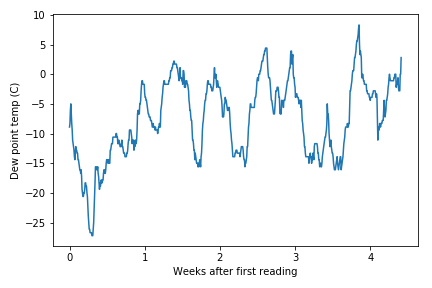
\includegraphics[width=3in]{polyfit_orig.png}
\end{center}


\item We want to form a polynomial regression of this data. That is, given $w = $ weeks and $d$ = dew readings, we want to find $\theta_1,...,\theta_p$ as the solution to
\begin{equation}
\underset{\theta\in \mathbb R^p}{\text{minimize}} \quad \tfrac{1}{2}\sum_{i=1}^m (\theta_1 + \theta_2 w_i + \theta_3 w_i^2 + \cdots + \theta_{p} w_i^{p-1} - d_i)^2.
\label{eq:polyfit0}
\end{equation}
Form $X$ and $y$ such that \eqref{eq:polyfit0} is equivalent to the least squares problem
\begin{equation}
\underset{\theta\in \mathbb R^p}{\text{minimize}} \quad \tfrac{1}{2}\|X\theta - y\|_2^2.
\label{eq:polyfit1}
\end{equation}
That is, for $w$ the vector containing the week number, and $y$ containing the dew data, form 
\[
X = \bmat
1 & w_1 & w_1^2&  w_1^3 &\cdots &w_1^{p-1}\\
\vdots& \vdots & \vdots & \ddots & \vdots\\
1 & w_m & w_m^2&  w_m^3 &\cdots &w_m^{p-1}\\
\emat.
\]

\end{itemize}
\begin{enumerate}
\item \emph{Linear regression.}
\begin{enumerate}
\item Write down the normal equations for problem \eqref{eq:polyfit1}. 

\item Fill in the code to solve the normal equations for $\theta$, and use it to build a predictor.
To verify your code is running correctly, the number after \texttt{check number} should be   $1.341$.


\item Implement a polynomial fit of orders $p = 1,2,3,10,100$, for the weather data provided. Include a figure that plots the original signal, overlaid with each polynomial fit. Comment on the ``goodness of fit" for each value of $p$.



\end{enumerate}
\item \emph{Ridge regression.} Oftentimes, it is helpful to add a \emph{regularization term} to \eqref{eq:polyfit1}, to improve stability.  In other words, we solve 
\begin{equation}
\underset{\theta\in \mathbb R^p} {\text{minimize}}\quad \tfrac{1}{2}\|X\theta - y\|_2^2 + \tfrac{\rho}{2} \|\theta\|_2^2.
\label{eq:polyfit2}
\end{equation}
for some $\rho > 0$. 
\begin{enumerate}
\item Again, write down the normal equations for \eqref{eq:polyfit2}. Your equation should be of form $A\theta =b$ for some matrix $A$ and vector $b$ that you specify.



\item Write the code for solving the ridge regression problem and run it. To verify your code is running correctly, the number after \texttt{check number} should be   $1.206$.

\item  Using $\rho = 1.0$,  plot the weather data with overlaying polynomial fits with ridge regression. Provide these plots for $p = 1,2,3,10,100$. Comment on the ``goodness of fit" and the stability of the fit, and also compare with the plots generated without using the extra penalty term. 


\end{enumerate}

\item \emph{Conditioning.}
\begin{enumerate}
\item An \emph{unconstrained quadratic problem} is any problem that can be written as
\begin{equation}
\minimize{\theta}\quad \frac{1}{2}\theta^TQ\theta + c^T\theta + r
\label{eq:quadratic_problem}
\end{equation}
for some symmetric positive semidefinite matrix $Q$, and some vector $c$ and some scalar $r$. Show that the ridge regression problem \eqref{eq:polyfit2} is an unconstrained quadratic problem by writing down $Q$, $c$, and $r$ in terms of $X$ and $y$ such that
\eqref{eq:quadratic_problem} is equivalent to \eqref{eq:polyfit2}. Show that the $Q$ you picked is positive semidefinite. 


\item In your code, write a function that takes in $X$ and $y$, constructs $Q$ as specified in the previous problem, and  returns the condition number of $Q$. Report the condition number $\kappa(Q)$ for varying values of $p$ and $\rho$, by filling in the following table. 
Here, $m = 742$ is the total number of data samples. Report at least 2 significant digits.
Comment on how much ridge regression is needed to affect conditioning.

\begin{center}
\begin{tabular}{|l||l|l|l|l|}\hline
p& $\rho = 0$   & $\rho = m$   &$\rho = 10m$   &$\rho = 100m$\\ 
\hline\hline
1&  &&&\\
\hline
2&  &&&\\\hline
5&  &&&\\\hline
10& &&&\\\hline
\end{tabular}
\end{center}






\item Under the \emph{same experimental parameters} as the previous question, run ridge regression for each choice of $p$ and $\rho$, and fill in the table with the mean squared error of the fit:
\[
\textbf{mean squared error} = \frac{1}{m}\sum_{i=1}^m (x_i^T\theta - y\idx{i})^2
\]
where $x_i$ is the $i$th row of $X$.
Comment on the tradeoff between using larger $\rho$ to improve conditioning vs its affect on the final performance. 


\begin{center}
\begin{tabular}{|l||l|l|l|l|}\hline
p& $\rho = 0$   & $\rho = m$   &$\rho = 10m$   &$\rho = 100m$\\ 
\hline\hline
1&  &&&\\
\hline
2&  &&&\\\hline
5&  &&&\\\hline
10& &&&\\\hline
\end{tabular}
\end{center}




\end{enumerate}
\item \emph{Forcasting.} Picking your favorite set of hyperparameters ($p$, $\rho$), forecast the next week's dew point temperature. Plot the forecasted data over the current observations. Do you believe your forecast? Why?








\end{enumerate}



\item \showpoints{2 pts } \emph{Logistic regression for Binary MNIST} 
\begin{enumerate}
\item \showpoints{0.5 pt}
What is the gradient of the logistic loss function 
\[
f(\theta) = -\frac{1}{m}\sum_{i=1}^m \log(\sigma(y_ix_i^T\theta)), \quad \sigma(s) = \frac{1}{1+e^{-s}}
\]
where $y_i \in \{-1,1\}$? (Hint: Check out problem 1 again.)






\item \textbf{Coding gradient descent.} Do \textbf{not} use  \texttt{scikit-learn} or other built in tools for this exercise. Please only use the packages that are already imported in the notebook. \footnote{This is to test your understanding of the basic machine learning concepts, like calculating accuracy and logistic loss; in the future you can use whatever tools you'd like.}

\begin{itemize}
\item Open \texttt{mnist\_logreg.ipynb}. We will use logistic regression to diffrentiate 4's from 9's, a notoriously tricky problem.
Run the first box to see what the data looks like.

\item In the second box I have set up the problem for you by pulling out the train and test set, selecting out only the data samples related to 4's and 9's. I have not altered the data in any other way. While other normalization tricks will help you improve the accuracy, for the purposes of this exercise we will forgo them, so that it's easy to compare everyone's solutions. 


 
\item Fill in the next box by providing code that will return the loss function value and the gradient. Make sure that everything is normalized, e.g. don't forget the $1/m$ term in the front of our loss function. Run the script.
If done correctly, you should see 
\begin{center}
\texttt{45.192, 12343.177}
\end{center}

\item Write a script that returns the classification accuracy given $\theta$. 
\item Use gradient descent to minimize the logistic loss for this classification problem. Use a step size of $10^{-6}$.

    \item \showpoints{1 pt} Run for 1500 iterations. In your report, give the plot of the train  loss and train/test misclassification rate, plotted as a function of \emph{iterations}. Report the final train and test accuracy values. 




\end{itemize}
 
\item \textbf{Coding stochastic gradient descent.} Do \textbf{not} use  \texttt{scikit-learn} or other built in tools for this exercise. Please only use the packages that are already imported in the notebook. Now, fill in the next box a function that takes in $\theta$ and a minibatch $\mathcal B$ as either a list of numbers or as an np.array, and returns the \emph{minibatch gradient}
\[
\nabla_\mB f(\theta) = \frac{1}{|\mB|}\sum_{i\in \mB} \nabla f_i(\theta)
\]
where $f_i(\theta)$ is the contribution to the gradient from datapoint $i$:
\[
f_i = -\log(\sigma(y_ix_i^T\theta)).
\]
Run the script. If done correctly, you should see the number 5803.5 printed out. 

\item Write a script to run stochastic gradient descent over logistic regression. When coding up the minibatching, make sure you cycle through an entire training set once before moving on to the next epoch. Additionally, use \texttt{time()} to record the runtime, and compare the performance of gradient descent and stochastic gradient descent, using a minibatch size of 50 data samples and running for 50000 iterations. Return a plot that compares the objective loss, train accuracy, and test accuracy between the two optimization methods, as a function of \emph{runtime}. Comment on the pros and cons of the two methods.


\textbf{Important} Remember that calculating the loss function and train/test accuracy requires making \emph{full passes} through the data. If you do this at each iteration, you will not see any runtime benefit between stochastic gradient descent and gradient descent. Therefore I recommend you log these values every 10 iterations for gradient descent, and every 100 iterations for stochastic gradient descent. 


\end{enumerate}

\end{enumerate}

\newpage

\section*{Challenge!}

\begin{enumerate}

%\item  \showpoints{1 pt} \emph{Advanced linear algebra and convex optimization.} 




\item \showpoints{1 pt.}  \emph{Gradient descent for ridge regression.} Consider the problem 
\begin{equation}
\minimize{x} \quad \overbrace{\underbrace{\frac{1}{2}\|Ax-b\|_2^2}_{=:f(x)} + \frac{\rho}{2}\|x\|_2^2}^{F(x)}
\label{eq:linreg}
\end{equation}
where $A\in \R^{m\times n}$ and $n > m$. Justify all answers.
\begin{enumerate}
\item Define $C=A^TA$. Recall that an eigenvalue of a symmetric matrix $C$ is $\lambda$ where $Cv = \lambda v$ for some vector $v$. Show that if $\lambda_{\max}^2$ is the largest eigenvalue of $C$ and $\lambda_{\min}^2$ the minimum eigenvalue of $C$, then for any vector $u$,
\[
\lambda_{\min}^2 \|u\|_2\leq \|Cu\|_2 \leq \lambda_{\max}^2 \|u\|_2.
\]
Hint: The \emph{eigenvalue decomposition} of a symmetric matrix can be written as $C = V\Lambda V^T$ where $V = \bmat v_1 & v_2 & \cdots & v_n\emat$ contain the eigenvalues $v_i$ of $C$, and $\Lambda = \diag(\lambda_1,\lambda_2,\cdots,\lambda_n)$ contain the corresponding eigenvalues $\lambda_i$. (That is, $Cv_i = \lambda_i v_i$.) Under certain conditions which we will just assume \footnote{eigenvalues must all have algebraic multiplicity = geometric multiplicity} then $V$ is an orthonormal matrix, e.g. $V^TV=VV^T = I$. Then, we can use this to form projections, e.g. pick any vector $u$. Then $VV^Tu = V^TVu = u$. 



\item Show that since $n > m$, then if $C = A^TA$ then $\lambda_{\min}(C) = 0$. Hint: The nonzero eigenvalues of $AA^T$ and of $A^TA$ are the same.


\item We say a function $f:\R^n\to\R$ is $L$-smooth if its gradient is $L$-Lipschitz, e.g. for some $L>0$,
\[
\|\nabla f(x) - \nabla f(y)\|_2 \leq L\|x-y\|_2,\quad \forall x,y.
\]
Is $f(x)$ as defined in \eqref{eq:linreg} $L$-smooth? What about  $F(x)$?




\item We say a function $f:\R^n\to\R$ is $\mu$-strongly convex if it is tangent to a quadratic function that is strictly under it; that is, for some $\mu > 0$, 
\[
f(x)-f(y) \geq \nabla f(y)^T(x-y)+\frac{\mu}{2}\|x-y\|_2^2,\quad \forall x,y.
\]
If this is only true for $\mu = 0$, we say $f$ is convex, but not strongly convex. 

Is the function $f(x)$ in \eqref{eq:linreg} $\mu$-strongly convex? What about  $F(x)$?
Hint: This problem requires less work if you first answer for $F(x)$, and then take $\rho = 0$ for $f(x)$. 




\item \emph{Linear convergence.} We will now show that gradient descent on minimizing $F(x)$ converges \emph{linearly.} First, recall that gradient descent iterates as 
\[
x^{(t+1)} = x^{(t)} - \alpha\nabla F(x^{(t)})
\]
for some step size $\alpha > 0$. 
\begin{enumerate}
\item Show that for any point $x^*$ where $\nabla F(x^*) = 0$,
\[
\|x^{(t+1)}-x^*\|_2 \leq c \|x^{(t)}-x^*\|_2
\]
for some $c < 1$. What is $c$?



\item Use this to argue that gradient descent on \eqref{eq:linreg} converges with  \emph{linear complexity}, e.g.  the error $f(x^{(t)}) - f(x^*) = O(c^t)$.
\footnote{It's a weird convention, but we say $O(c^t)$ is a linear rate because the loglog graph looks linear. I don't make the rules, I just share them with you.}




\end{enumerate}
\end{enumerate}

\item \showpoints{1pt} \emph{Linear regression without strong convexity still gets linear convergence.} Now consider linear regression with $A = \bmat 1 & 1 \\ 1 & 1 \emat$,  $b = \bmat 1 \\ -1\emat $, and $\rho = 0$ (no ridge). 
That is, we consider only 
\[
f(x) = \frac{1}{2}\|Ax-b\|_2^2.
\]
\begin{enumerate}
\item \emph{Linear algebra.} For a matrix $A$, the \textbf{nullspace} of $A$ is the set 
\[
\vnull(A) = \{x : Ax = 0\},
\]
and the \textbf{range} of $A$ is the set 
\[
\range(A) = \{Ax \text{ for any } x\}.
\]
Show that for 
\[
u = \bmat 1 \\ -1 \emat, \qquad v = \bmat 1 \\ 1 \emat,
\]
then $u\in \vnull(A)$ and $v\in \range(A)$.



\item 
\emph{Linear decomposition theorem part 1.}
Show that for \emph{any} vector $u\in \vnull(A)$ and $v\in \range(A^T)$, it must be that $u^Tv = 0$.



\item 
\emph{Linear decomposition theorem part 2.}
Argue also that for \emph{any} vector $x$, there exist some $u\in \vnull(A)$ and $v\in \range(A^T)$ where $x = u+v$. Do this by providing two matrices $P$ and $Q$ where $Px = u$ and $Qx = v$, using   $A = \bmat 1 & 1 \\ 1 & 1 \emat$. (This matrix will be unique.)
 

\item \emph{Linear regression doesn't pick up nullspace components.} Suppose $x^{(0)} = \bmat 0 \\ 0 \emat$.   Now we run the gradient descent method
\begin{equation}
x^{(t+1)} = x^{(t)} - \alpha \nabla f(x^{(t)})
\label{eq:gd1}
\end{equation}
to get $x^{(1)}$, $x^{(2)}$, ...

Show that using this initial point,   $Qx^{(t)}=0$ for \emph{all} $t$, where $Q$ is the matrix computed in the previous question.

\item \emph{Linear regression doesn't pick up nullspace components, another example.} 
Now suppose that for some $x^{(0)}$, $Qx^{(0)} = r\neq 0$.  Again, we run the gradient descent method.
Show that $Qx^{(t)} = r$ for all $t$. (That is, $r$ does not depend on $t$!)





\item Now consider a \emph{reduced gradient descent problem}, where we minimize over a scalar variable $v$
\[
\minimize{v\in \R} \; g(v) = \frac{1}{2}\|ASv-Pb\|_2^2, \quad S = \frac{1}{\sqrt{2}}\bmat 1 \\ 1\emat.
\]
Argue that, using gradient descent
\[
v^{(t+1)} = v^{(t)} - \alpha \nabla g(v^{(t)}),
\]
the iterates $x^{(t)} = Sv^{(t)}$ are exactly those outputted by \eqref{eq:gd1} where $x^{(0)} = Sv^{(0)}$.

Hint: Start by showing that $SS^T\nabla f(x) = \nabla f(x)$.



\item Finally, show that $g(v)$ is strongly convex in $u$. 




\item Show that for this specific choice of $A$, gradient descent converges linearly, e.g. $f(x^{(t)}) - f(x^*) = O(c^t)$, and carefully state what $c$ is.




\item Now consider \emph{any} matrix $A$. Argue that this entire problem basically shows that gradient descent, minimizing linear regression, will \emph{always} converge at a linear rate, and describe what $c$ is.


\end{enumerate}



\end{enumerate}

\end{document}